\documentclass[14pt]{extarticle}
\usepackage[
left=25mm,
top=20mm,
right=15mm,
bottom=20mm,
]{geometry}

%\usepackage{graphicx}
\usepackage[pdftex]{graphicx}
\usepackage[utf8x]{inputenc}
\usepackage[russian]{babel}
\usepackage[T1]{fontenc}
\usepackage{float}
\usepackage{listings}
\usepackage{cite}
\usepackage{hyperref}
\usepackage{etoolbox}
\usepackage{indentfirst}
\usepackage[linesnumbered,boxed]{algorithm2e}
%\sloppy

\lstset{
	sensitive=true,
	basicstyle=\small,
	keywordstyle=\color{black},
	commentstyle=\scriptsize\rmfamily,
	keywordstyle=\ttfamily\underbar,
	identifierstyle=\ttfamily,
	basewidth={0.5em,0.5em},
	columns=fixed,
	fontadjust=true,
	literate={->}{{$\to$}}1
}

\makeatletter
%\renewcommand{\@biblabel}[1]{#1.} % Заменяем библиографию с квадратных скобок на точку:
\makeatother
\gappto\captionsrussian{\renewcommand{\contentsname}{Оглавление}}
\renewcommand\baselinestretch{1.5}
\renewcommand{\lstlistingname}{Листинг}

\begin{document}
	
	\begin{titlepage}
	\thispagestyle{empty}
		\def\baselinestretch{1.0}
		\begin{center}
			{САНКТ-ПЕТЕРБУРГСКИЙ ГОСУДАРСТВЕННЫЙ УНИВЕРСИТЕТ \\ \vskip 0.3em {\large Математико-механический факультет \\ \vskip 0.7em{\large Кафедра системного программирования \\}}}
			\vspace*{0.15\textheight}
			{\large Гудиев Артур Владимирович}
			
			\vskip 2em
			{\LARGE Реализация примитвов и оконного менеджера для построения пользователских интерфейсов на языке PostScript}
			
			\vskip 1em
			{\large Дипломная работа} \\
			\vskip 2em
			{\normalsize \raggedleft 
				Допущена к защите.\\
				Зав. кафедрой:\\
				д.ф.-м.н., проф. А.Н. Терехов
				\\[2em]
				Научный руководитель:\\
				к.ф.-м.н. Д.Ю. Булычев
				\\[2em]
				Рецензент:\\
				Д.В. Кознов
				\\[2em]
				%Неизвестно \\
				\vspace*{0.08\textheight}
				{\centering Санкт-Петербург \\ 2015}
			}
		\end{center}
	\end{titlepage}
	\begin{titlepage}
		\thispagestyle{empty}
		\def\baselinestretch{1.0}
		\begin{center}
			{SAINT-PETERSBURG STATE UNIVERSITY \\ \vskip 0.3em {\large Mathematics \& Mechanics Faculty \\ \vskip 0.7em{\large Department of Software Engineering \\}}}
			\vspace*{0.15\textheight}
			{\large Artur Gudiev}
			
			\vskip 2em
			{\LARGE Window manager and GUI primitives for user interface implementation in PostScript}
			
			\vskip 1em
			{\large Graduation Thesis} \\
			\vskip 2em
			{\normalsize \raggedleft 
				Adnitted for defence.\\
				Head of the chair:\\
				professor  Andrey Terekhov
				\\[3em]
				Scientific supervisor:\\
				Dmitri Boulytchev
				\\[3em]
				Reviewer:\\
				Dmitri Koznov
				\\[2em]
				%Неизвестно \\
				\vspace*{0.08\textheight}
				{\centering Saint-Petersburg \\ 2015}
			}
		\end{center}
	\end{titlepage}
	
	\setcounter{page}{3}
	\tableofcontents
	
	%\thispagestyle{empty} 
	\pagebreak
	
	
	\section*{Введение}
	\addcontentsline{toc}{section}{Введение}
	PostScript - это графический интерпретируемый язык программирования, создавашийся с целью представления графики в машинонезависимой форме. Посредством графических операторов языка PostScript можно отобразить на экране прямые и кривые линии, залить цветом область, определить область рисования, задать графические параметры.  
	
	Графический интерфейс пользователя - это разновидность пользовательского интерфейса, в котором элементы интерфейса представлены в виде графических примитивов. Визуальные интерфейсы пользователя упрощают работу с программами, делая ее наглядной. Язык PostScript обладает базовыми графическими возможностями для отображения внешнего вида графических интерфейсов.
	
	Оконный менеджер — это приложение, управляющее размещением окон и определяющая их внешний вид в оконной системе графического интерфейса. Оконные менеджеры работают на основе существующей оконной системы. Кроме того оконный менеджер включает в себя и визуальные эффекты, проявляющиеся во время работы с окнами. Обычно оконный менеджер привязан к конкретной операционной системе. Язык PostScript позволяет нарисовать такие объекты, как элементы графического интерфейса пользователя и визуальные эффекты оконного менеджера.
	
	Ранее в рамках проекта лаборатории JetBrains был реализован интерпретатор графического языка PostScript. Однако с его помощью было трудно создавать графические интерфейсы и оконный менеджер из-за того, что, например, в PostScript не поддерживается механизм обработки событий. Для упрощения реализации этой возможности планируется расширить язык PostScript. Данная работа ведется по трем направлениям: оптимизация интерпретатора (Д. Поздин), обработка событий (Р. Макулов) и реализация графических примитивов и оконного менеджера (А. Гудиев).
	
	Целью данной дипломной работы является реализация графических примитивов и оконного менеджера для создания пользовательских интерфейсов на языке PostScript.
	
	\pagebreak
	\section{Обзор}
	\subsection{ Описание существующих решений }
		\subsubsection*{Qt Quick}
		%\label{sec:qtquick}
		%\addcontentsline{toc}{subsubsection}{\nameref{sec:qtquick}}

Пользовательские интерфейсы разработанные в Qt Quick создаются как прямоугольные элементы в визуальном дереве. Технология ограничена набором элементов сфокусированных на взаимодействии через прикосновения и жесты. Qt Quick вводит новую концепцию логики моделирования приложений, используя иерархическую машину состояний. Кроме того, переходы и богатый набор анимаций (tweens) облегчают создание богатых пользовательских интерфейсов.

Большой проблемой для дизайнеров было участие в процессе разработки с Qt и C++. C, в конце концов, является языком низкого уровня ориентированным на системное программирование. Qt Quick был разработан с нуля, чтобы заполнить этот пробел. Как предметно-ориентированный язык он специально ориентирован на создание пользовательских интерфейсов. Это устанавливает декларативный слой поверх JavaScript, который похож на каскадные таблицы стилей (CSS). В Qt не будут беспокоить приведение типов, указатели и время жизни объектов. Вместо этого, в центре внимания находится создание богатых пользовательских интерфейсов. 		
		
		\subsubsection*{Java Swing}
	    %\label{sec:javaswing}
		%\addcontentsline{toc}{subsubsection}{\nameref{sec:javaswing}}
				
				Компания Sun разработала набор графических компонентов под названием Swing. Компоненты Swing полностью написаны на Java. Для отрисовки используется 2D, что принесло с собой сразу несколько преимуществ. На Swing легко создавать новые компоненты, наследуясь от существующих. Стала возможной поддержка различных стилей и скинов. 

Благодаря простоте использования, богатой документации и гибкости компонентов Swing стал, пожалуй, самым популярным графическим фреймворком в Java. На его базе появилось много расширений, таких как SwingX, JGoodies, которые значительно упрощают создание сложных пользовательских интерфейсов. Практически все популярные среды программирования Java включают графические редакторы для Swing-форм, что облегчает освоение Swing.
		\subsubsection*{Недостатки существующих решений }
		%\label{sec:decisions}
		%\addcontentsline{toc}{subsubsection}{\nameref{sec:decisions}}
	
		К недостаткам Swing можно отнести медленную работу при окнах с большим количеством элементов.
		 
	\subsection{Описание используемых инструментов }
		
		\subsubsection*{JVM}
		%\label{sec:jvm}
		%\addcontentsline{toc}{subsubsection}{\nameref{sec:jvm}}
	
		Виртуальная машина Java (сокращенно JVM) - основная часть среды выполнения для Java, так называемой Java Runtime Environment (JRE). Программы на языке Java компилятором Java (javac) переводятся в байт-код Java. Виртуальная машина Java исполняет байт-код. В настоящее время JVM получила широкое распространение. Ее реализация есть для многих операционных систем, что делает программы, написанные на Java, кроссплатформенными. Интерпретатор PostScript, реализованный в рамках проекта JetBrains, написан на языке Java.
		\subsubsection*{Java Swing и Java AWT}
		%\label{sec:swingawt}
		%\addcontentsline{toc}{subsubsection}{\nameref{sec:swingawt}}
		Java Swing и Java AWT- это библиотеки языка Java, с помощью которых в реализованном интерпретаторе строится путь рисования, отображаются шрифты, задаются параметры графической среды исполнения такие, как цвет, ширина линии, способ соединения отрезков. 
		\subsubsection*{ Реализованный интерпретатор PostScript }
		%\label{sec:interpreter}
		%\addcontentsline{toc}{subsubsection}{\nameref{sec:interpreter}}
		Интерпретатор PostScript, реализованный в рамках проекта JetBrains, написан на Java. Он состоит из следующих пакетов: парсер (parser), среда исполнения (runtime) и интерпретатор (interpreter). 
		
		Парсер разбивает входной поток на токены согласно синтаксису PostScript и записывает их в виде процедуры.
		
		Среда исполнения содержит в себе реализацию основных операторов (например, add, show, if, for ...) и объектов, то есть их значений, типов и атрибутов. Среда исполнения содержит также и класс AVL-дерева, используемый в словарях, стеки, виртуальную память, в которой хранятся значения сложных объектов и графическую среду исполнения. В графической среде исполнения описаны классы отображения результата программы на экране, матрица преобразования системы координат, класс пути, с помощью которого строится изображение, класс снимка графического состояния, используемый при сохранении или восстановлении графического состояния и набор графических параметров (например, цвет, ширина линии, форма концов отрезка ... ).
		
		Интерпретатор передает парсеру программу PostScript, получает в качестве результата процедуру, кладет ее на стек исполнения и запускает выполнение стека исполнения.
		
	\subsection{ Проект рабочей группы интерпретатора PostScript }
Задача реализации интерпретатора графического языка PostScript решается в рамках проекта компании JetBrains. 
		
		Проект можно разделить на задачи:
		\begin{itemize}
		\item оптимизация интерпретатора;
		\item добавление механизма обработки событий;
		\item реализация примитивов и оконного менеджера.
		\end{itemize}	
	
	\pagebreak
	\section{Примитивы графической библиотеки}
	\subsection*{Структура графических примитивов}
		Код графческой библиотеки языка PostScript содержится в файле  glib.ps. В нем создается словарь gelements. У каждого примитива есть свой номер, по которому он хранится в словаре gelements. 
		
		У графических примитивов реализовано отношение наследования. Общий предок у всех - объект сцена (scene). У каждого примитива есть дети-примитивы. Номера детей хранятся в поле-массиве children.
		
		Каждому графическому примитиву соответствуют два файла - файл с описанием объекта и файл с процедурой отрисовки примитива. (Например, для кнопки - это button.ps и paintButton.ps). 
		
		В файле первом есть два конструктора - абсолютный и относительный. У каждого примитива есть свои координаты и размеры. Если координаты задаются относительно родителя, то вызывается относительный контсркутор. Если примитив задается абсолютными координатами, тогда вызывается абсолютный. Например, пусть есть окно с левым нижним концом в точке (0,0), высотой 1000 и шириной 1000. Пусть от окна наследуется кнопка с левым нижним концом в (200, 300), длиной 400 и шириной 500. 
		
		Тогда абсолютный контсруктор -
		200 300 400 500 ... button
		
А относительный - 
		0.2 0.3 0.4 0.5	... relButton.
		
		
Относительные координаты хороши тем, что при изменении размеров или сдвиге родителя, они не изменяются.

Каждому примитиву можно добавить событие - процедуру PostScript. Их может быть несколько. У каждого графического объекта есть словарь eventProcDict, в нем хранятся процедуры, которые вызываются при событии у объекта. 
	
	\subsection*{Кнопка}
	%\label{sec:button}
	%\addcontentsline{toc}{subsection}{\nameref{sec:button}}
	Кнопка - примитив, у которого вызывается заданное событие по нажатию. У кнопки есть два варианта отрисовки: с обычной и с нажатой кнопкой. В процедуре рисования проверяется, нажата ли кнопка. Если да, то рисуется затемненная кнопка без тени, а иначе светлая с тенью.
		\begin{figure}[h]
		\begin{center}
		\begin{minipage}[h]{0.4\linewidth}
		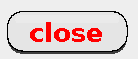
\includegraphics[width=180pt]{pictures/close1.png}
		\caption{ Кнопка} %% подпись к рисунку
		\label{ris:b1} %% метка рисунка для ссылки на него
		\end{minipage}
		\hfill 
		\begin{minipage}[h]{0.4\linewidth}
		
\includegraphics[width=180pt]{pictures/close2.png}
		\caption{Нажатая кнопка}
		\label{ris:b2}
		\end{minipage}
		\end{center}
		\end{figure}	
		
	\subsection*{Флажок}
	Примитив флажок позволяет вызывать заданные процедуры при снятии и задании флага. В процедуре отрисовки проверяется, стоит ли флаг. Если стоит, то рисуется квадратик в области.
		\begin{figure}[h]
		\begin{center}
		\begin{minipage}[h]{0.4\linewidth}
		
\includegraphics[width=180pt]{pictures/checkBox1.png}
		\caption{Флажок} %% подпись к рисунку
		\label{ris:b1} %% метка рисунка для ссылки на него
		\end{minipage}
		\hfill 
		\begin{minipage}[h]{0.4\linewidth}
		
\includegraphics[width=180pt]{pictures/checkBox2.png}
		\caption{Отмеченный флажок}
		\label{ris:b2}
		\end{minipage}
		\end{center}
		\end{figure}	
			
		
	\pagebreak		
	\subsection*{Поле со списком}
	Примитив поле со списком позволяет выбрать один из заданных вариантов. Данный примитив состоит из поля, в котором отображается выбранный вариант, и списка со всеми вариантами. Изначально список свернут, отображается только поле. При нажатии на поле список раскрывается, отображаются все варианты. При следующем нажатии по координатам клика проверяется, был ли выбран какой-нибудь вариант, и если да, то вычисляется, какой именно. После этого список сворачивается. 
	
		\begin{figure}[h]
		\begin{center}
		\begin{minipage}[h]{0.4\linewidth}
		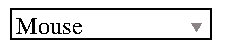
\includegraphics[width=180pt]{pictures/comboBox1.png}
		\caption{ Поле со списком} %% подпись к рисунку
		\label{ris:b1} %% метка рисунка для ссылки на него
		\end{minipage}
		\hfill 
		\begin{minipage}[h]{0.4\linewidth}
		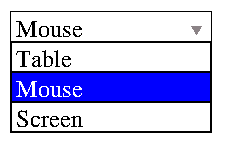
\includegraphics[width=180pt]{pictures/comboBox2.png}
		\caption{Раскрытое поле со списком}
		\label{ris:b2}
		\end{minipage}
		\end{center}
		\end{figure}
		
	\subsection*{Список}
	Список также предоставляет возможность выбора одного из имеющихся вариантов. Отличие списка от поля со списком в том, что в первом список всегда развернут, то есть все варианты постоянно отображаются. Выбранный вариант рисуется на синем фоне. При нажатии на список проверяется, на каком варианте произошел клик. Затем старый выбранный вариант уже отображается на белом фоне, а новый выбранный - на синем. 
		\begin{figure}[h]
		\center{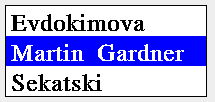
\includegraphics[width=180pt]{pictures/listBox.png}}
		\caption{Список}
		\label{ris:image}
		\end{figure}	
	
	\subsection*{Метка}
		Примитив метка отображает текст на экране. При необходимости можно самостоятельно задать размер шрифта и цвет. Для этого нужно в словаре метки поставить по ключу isAttached значение true, и задать необходимые значения ключам kegel и color. 
		\begin{figure}[h]
		\center{
\includegraphics[width=180pt]{pictures/label.png}}
		\caption{ Метка }
		\label{ris:image}
		\end{figure}	

	\subsection*{Поле редактирования}
	%\label{sec:textField}
	%\addcontentsline{toc}{subsection}{\nameref{sec:textField}}
		Поле редактирования - это примитив, предназначенный для ввода текста. Изначально в поле ничего не отображается. При нажатии на поле, появляется курсор. Сразу после ввода символы появляются на экране. Курсор можно сдвигать влево и вправо, в начало и конец строки. Напечатанные символы можно удалять. Если введенная строка превышает ширину поля, то вычисляется, какая подстрока отображается на экране. 
		\begin{figure}[h]
		\center{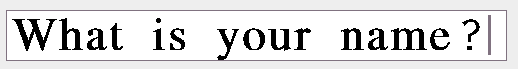
\includegraphics[width=180pt]{pictures/textField.png}}
		\caption{ Поле редактирования }
		\label{ris:image}
		\end{figure}	
	\subsection*{Радиокнопка}
		Радиокнопка - это кнопка, которая может находиться в включенном или выключенном состоянии. При отрисовке радиокнопки проверяется, в каком она состоянии, и в зависимости от этого отображается включенная или выключенная радиокнопка.
		\begin{figure}[h]
		\begin{center}
		\begin{minipage}[h]{0.4\linewidth}
		
\includegraphics[width=90pt]{pictures/toggleButton1.png}
		\caption{ Включенная радиокнопка} %% подпись к рисунку
		\label{ris:b1} %% метка рисунка для ссылки на него
		\end{minipage}
		\hfill 
		\begin{minipage}[h]{0.4\linewidth}
		
\includegraphics[width=90pt]{pictures/toggleButton2.png}
		\caption{Выключенная радиокнопка}
		\label{ris:b2}
		\end{minipage}
		\end{center}
		\end{figure}
		
	\subsection*{Окно}
	Примитив окно позволяет хранить и отображать в себе другие примитивы. У окна можно динамически изменять размеры. Для этого нужно подвести курсор к границе окна, курсор при этом должен поменяться, затем нажать и расстянуть или сжать окно до нужных размеров. При этом у окон задан минимальный размер, меньше которого сжать не получится. Для изменения курсора был введен новый оператор cursor. Окно также можно и перемещать. Для этого нужно зажать верхнюю область окна, и перенести курсор вместе с окном в нужное место. К окну автоматически добавляются служебные примитивы: метка-надпись в верхней части окна и кнопка закрытия. Кнопка закрытия удаляет из словаря графических притивов gelements само окно и всех его потомков.
		\begin{figure}[h]
		\center{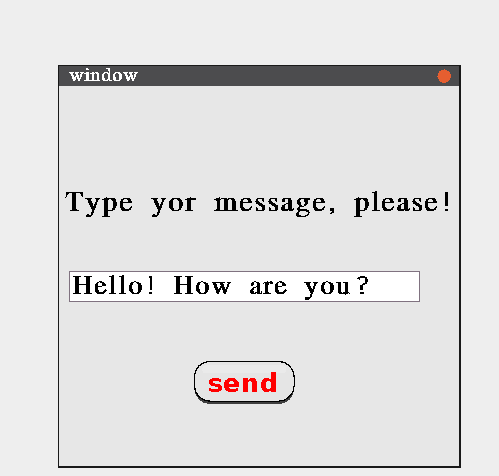
\includegraphics[width=180pt]{pictures/window.png}}
		\caption{ Окно }
		\label{ris:image}
		\end{figure}	
	\pagebreak
	
	\section{Реализация оконного менеджера}
	\subsection{ Оконная система }
	В программе может быть несколько окон, перекрывающих друг друга. Изначально все окна отображаются в том порядке, в каком они создавались. Но далее, если нажать на произвольное окно, то оно оказывается в фокусе. В графической библиотеке glib.ps в словаре gelements создается создается элемент focusedElement. Изначально это сцена. Но потом при нажатии на произвольный примитив, focusedElement становится равным выбранному примитиву. Если на окно нажали, то оно помимо того, что становится в фокусе, ещё и в списке детей родителя ставится последним. Это означает, что оно будет отображаться поверх остальных детей родителя, так как они рисуются в порядке списка.
	\subsection{ Архитектура оконного менеджера}
	Оконный менеджер хранит в себе очередь событий (EventQueue), очередь примитивов (PrimitiveQueue), время последней перерисовки (lasttime). Оконный менеджер принимает запросы на перерисовку и решает, стоит ли рисовать заново все примитивы. Это помогает избежать частых перерисовок.
	
	К оконному менеджеру можно добавить процедуры PostScript для отображения визуальных эффектов. В частности, сейчас добавлено событие волна: при нажатии правой кнопки мыши происходит эффект волны. 
	\pagebreak
	\section{Тестирование и демонстрационный пример}
	Ниже приведен демонстрационный пример, содержащий в себе примитивы.
 \linebreak

	\lstset{language=PostScript}          % Set your language (you can change the language for each code-block optionally)

\begin{lstlisting}[frame=single]  % Start your code-block

(graphicsEngine/basics/glib.ps) (r) file run

300 750 250 50 (Welcome! )  scene << >>    labelField pop
150 700 250 50 (Fill in this form, please. )  scene << >>    labelField pop

30 555 250 35 (Your name )  scene << >>    labelField pop
175 550 300 35  (TextField)    scene <<>>    textField pop

30 505 250 35 (Group )  scene << >>    labelField pop
175 500 100 35  (TextField)    scene <<>>    textField pop

30 435 250 35 (Education )  scene << >>    labelField pop
215 430 100 50 [ (Full-time) (Part-time) ] 1 scene << >> listBox pop

30 365 250 35 (Faculty )  scene << >>    labelField pop
200 365 350 30 [(Mathematics and Mechanics) (Physics) (Applied Mathematics) 
                 (Chemistry) ] 0  scene <<  >> comboBox pop

190 300 16  ( I want to get results)   scene << >> checkBox pop

30 105 250 35 (Error checking)  scene << >>    labelField pop
50 40 116 50 (On) (Off)  scene <<  >> toggleButton pop

500 25 120 40   (close) scene <</CLICK [{

  /messageWindow    370 140 250 150  scene << >> window def
  messageWindow /wLabel get /label (message) put
  390 215 250 30 (Do you want to save? )  messageWindow << >>    labelField pop
  430 165 50 25   (yes) messageWindow <</CLICK [{pop quit}[]] >>  button pop
  500 165 50 25   (no)  messageWindow 
  <</CLICK [{/CLOSE findAncestorWithEventType}[]] >> button pop 
                                
                                }[]] >> button pop
repaintAll
showpage
\end{lstlisting}
	В начале подключается библиотека графчиеской библиотеки. 
	Затем создается надпись "Welcome!" и "Fill in this form, please."
	
	После этого создаются напдись "Your name" и поле для ввода своего имени.
	
	Также вызывается контсруктор для надписи "Group" и поле для ввода номера своей группы. 
	
	Затем создается надпись "Education" и список для выбора формы обучения.
	
	Аналогично с надписью "Faculty" и полем со списком для выбора факультета.
	
	Ниже создается флажок с текстом "I want to get results" для подтверждения того, что пользователь хочет получить результат.
	
	После этого создается надпись "Error checking" и радиокнопка с надписями On и Off. 
	
	В конце создается кнопка Close, при нажатии которой появляется окно с вопрос, хочет ли пользователь сохранить результат.
	
	\begin{figure}[h]
		\begin{center}
		\begin{minipage}[h]{0.4\linewidth}
		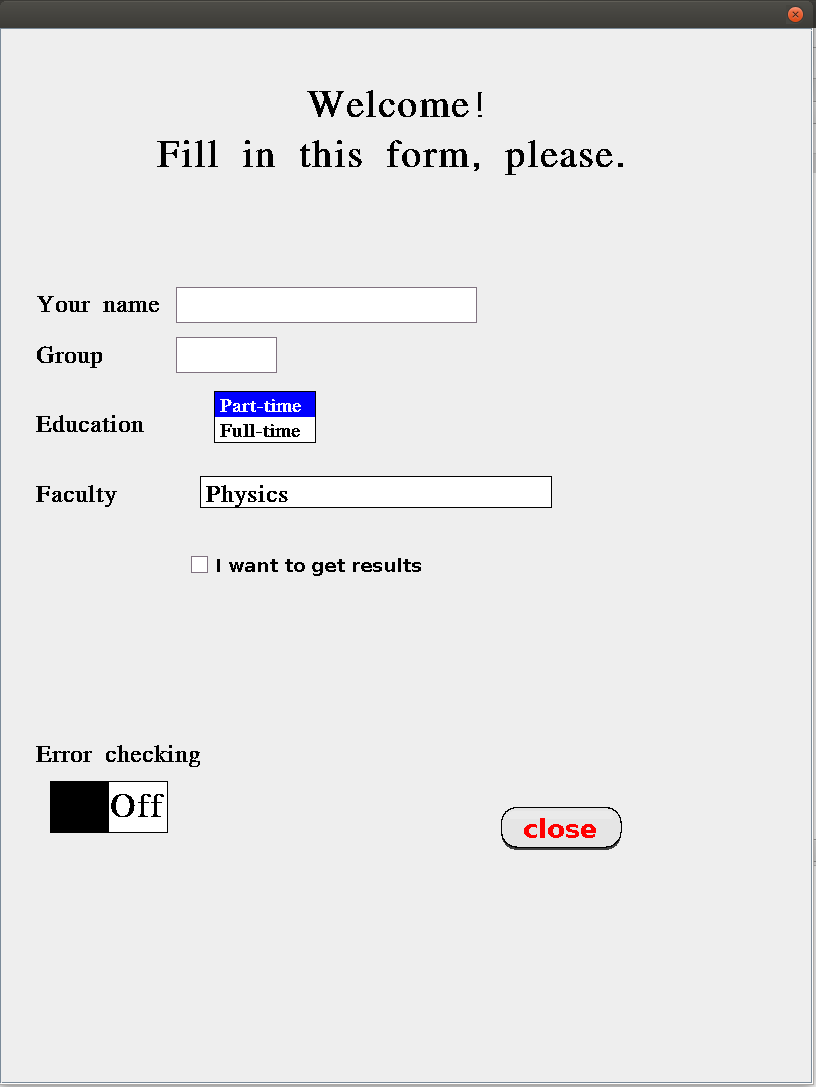
\includegraphics[width=230pt]{pictures/demo11.png}
		\caption{ Пустая форма} %% подпись к рисунку
		\label{ris:demo1} %% метка рисунка для ссылки на него
		\end{minipage}
		\hfill 
		\begin{minipage}[h]{0.4\linewidth}
		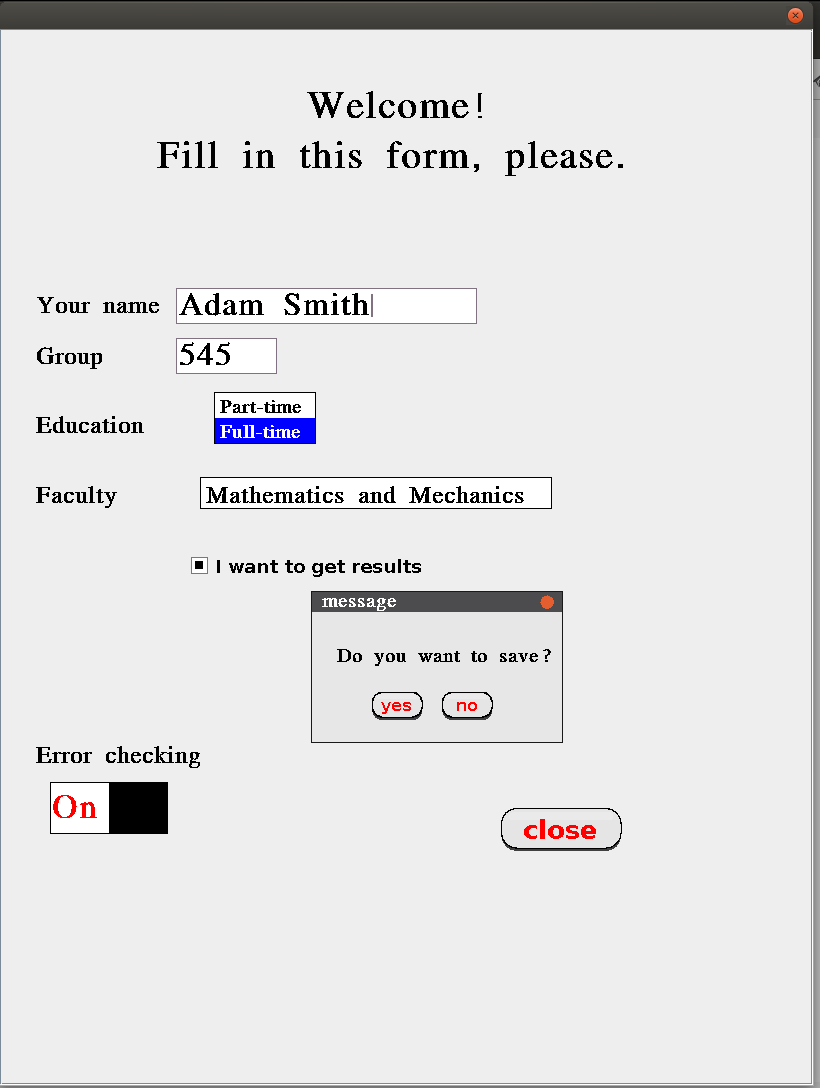
\includegraphics[width=230pt]{pictures/demo12.png}
		\caption{Заполненная форма}
		\label{ris:demo2}
		\end{minipage}
		\end{center}
		\end{figure}
		
	Код программы можно посмотреть в Приложении1.
	
	\pagebreak
	\section*{Заключение}
	\addcontentsline{toc}{section}{Заключение}
	
	В рамках дипломной работы получены результаты, перечисленные ниже.
	\begin{itemize}
		\item Добавлены следующие примитивы в графическую библиотеку  PostScript: кнопка, флажок, поле со списком, список, метка, поле редактирования, радиокнопка, окно.
		\item Реализован оконный менеджер, интегрированный с графической библиотекой.
		\item Проведено тестирование оконного менеджера на демонстрационном примере.
	\end{itemize}
	

	
	\pagebreak
	\bibliographystyle{ugost2008ls}
	
	
	\begin{thebibliography}{}
		
		\bibitem{PLRM}
		Спецификация языка Postscript. PostScript Language reference. \\
		Adobe Systems. 1999\\
		\url{http://www.adobe.com/products/postscript/pdfs/PLRM.pdf}
		
		\bibitem{jvms}
		Tim Lindholm, Frank Yellin, Gilad Bracha, Alex Buckley.
		The Java Virtual Machine Specification.
		Java SE 7 Edition, 2013. \\
		\url{docs.oracle.com/javase/specs/jvms/se7/jvms7.pdf}
		
		\bibitem{cormen}
		Томас Х. Кормен, Чарльз И. Лейзерсон, Рональд Л. Ривест, Клиффорд Штайн.
		Алгоритмы: построение и анализ.
		Второе издание, 2006
		
	\end{thebibliography}
\end{document}
